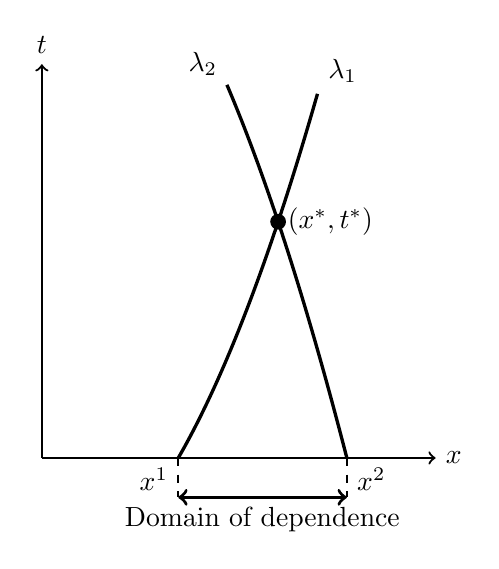
\begin{tikzpicture}
  \draw[thick,->](0,0)--(5,0) node [right] {$x$};
  \draw[thick,->](0,0)--(0,5) node [above] {$t$};
  % t1 = 0.5*x**2 + c1
  % t2 = -0.5*x**2 + c2
  % -> c1 = -1.5 ; c2 = 7.5
  % \draw[domain=1.7320508:3.5,smooth,variable=\x,Purple,very thick] plot ({\x},{0.5*\x*\x-1.5}) node [above right] {$t=\frac{x^2-3}{2}$};
  % \draw[domain=2.35:3.872983,smooth,variable=\x,Green,very thick] plot ({\x},{-0.5*\x*\x+7.5});
  \draw[domain=1.7320508:3.5,smooth,variable=\x,very thick] plot ({\x},{0.5*\x*\x-1.5}) node [above right] {$\lambda_1$};
  \draw[domain=2.35:3.872983,smooth,variable=\x,very thick] plot ({\x},{-0.5*\x*\x+7.5});
  % \node[left,Green] at (2.35,5) {$t=-\frac{x^2-15}{2}$};
  \node[left] at (2.35,5) {$\lambda_2$};
  \draw[<->,very thick] (1.7320508,-0.5) -- (3.872983,-0.5) ;
  \draw[dashed,thick]  (1.7320508,0) node [ below left] {$x^1$}-- (1.7320508,-0.5);
  \draw[dashed,thick]  (3.872983,-0.) node [ below right] {$x^2$} -- (3.872983,-0.5);
  \node[below] at (2.80,-0.5) {\text{Domain of dependence}};
  \fill[black] (3,3) circle (0.1) node [right] {$(x^*,t^*)$};
\end{tikzpicture}
%%% Local Variables:
%%% mode: latex
%%% TeX-master: "../../mainManuscript"
%%% End:
